\chapter{Background}
\label{chap:background}
%This is Chapter~ \ref{chap:background} and cite test \cite{Knight:1986:AMF:319838.319854, Sohi:1995:MP:225830.224451, Hammond:1998:DSS:291069.291020}. 


\section{The NVIDIA Jetson TX2}
The NVIDIA Jetson TX2 is a GPU platform targeted at power constrained mobile application. it is designed as an System
on Chip(SoC) which incorporates a quard-core 2.0-GHz 64-bit ARM-v8 A57 processor, a dual-core 2.0-GHz superscalar ARMv8 Denver processor and an integrated Pascal GPU. There are 2MB L2 caches, one shared by the four A57 cores and on shared by the two Denver cores. The GPU has two streaming multiprocessors (SM), each provides 128 1.3-GHz cores that share a 512-KB L2 cache. The six CPU cores and integrated GPU share 8 GB of 1.866-GHz DRAM memory.
 Fig. \ref{fig:fig_2_1} shows the example.
\begin{figure}[!h]
    \centering
    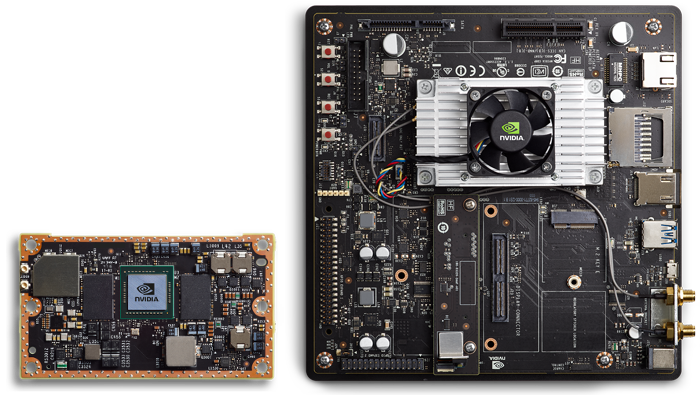
\includegraphics[scale=0.4]{image/jetson_tx2.png}
    \caption{The NVIDIA Jetson TX2 development board}
    \label{fig:fig_2_1}
\end{figure}

\section{Virtualization}
Virtualization refers  to the act of creating a virtual (rather than physical) version of something, includeing  virtual computer hardware platforms, storage devices, and computer network resources. it is a technique that use software to simulate the existence of hardware.
Traditional computing does not allow software to readily share hardware resources. Virtualization
overcomes that limitation by allowing users to run more than one software stack within each virtual system on single physical machine.

This can get greater efficiency of hardware. A virtual computer systems is known as
“virtual machine” (VM): an isolated software machine with an operating system and application
inside. Putting multiple virtual machines on a single computer enables several operating systems and
applications to run on one physical machine. A thin layer of software called a hypervisor which
manages the virtual machines at a physical machine and dynamically allocates computing resources like common processo, memory, I/O and storage to
each virtual machine as needed. 

Early virtualization efforts relied on software emulation to replace hardware functionality. But
software emulation is a slow and inefficient process.

There are three types of virtualization. First is full virtualization, second is para virtualization and third is hardware-assisted virtualization.

\begin{itemize}
    \item full virtualization: The operation system inside the virtual machine  is not aware that it is in a virtualized environment and requires no modification. 
        It use software to emulate all device operation and device driver can be directly installed in the virtual machine. However there are performance overhead and result in performance degradation.
    \item para virtualization : The operation system inside the virtual machine is aware that it is in a virtualized environment and 
        some of components are replaced with optimized one to gain better performance.
    \item hardware-assisted virtualization: An approach  that enables efficient full virtualization using help from hardware capabilities, primarily from the host processors. 
        while the guest must using the same instruction set as the host machine. Hardware-assisted virtualization was added to x86 processors (Intel VT-x or AMD-V) in 2005 and 2006 (respectively).
        Hardware-assisted virtualization reduces the maintenance overhead of paravirtualization as it reduces (ideally, eliminates) the changes needed in the guest operating system. It is also considerably easier to obtain better performance.
\end{itemize}

\section{GPU and NVIDIA CUDA}

Graphics Processing Unit (GPU) is a specialized electronic circuit designed to rapidly manipulate and alter memory to accelerate the creation of images in a frame buffer intended for output to a display device, e.g. personal computers, workstations, game consoles, embedded systems, and some mobile phones. In a personal computer, a GPU can be present on a video card, or it can be embedded on the motherboard, or in certain CPUs, on the CPU die. The term GPU was popularized by Nvidia in 1999. It was presented as a ``single-chip processor with integrated transform, lighting, triangle setup/clipping, and rendering engine''.

The difference between CPU and GPU is their operation method. The CPU consists few cores that used to optimize the sequential sequence processing, like branch condition. The GPU contains thousands of smaller cores to execute the processing of multiple tasks simultaneous. GPUs can be more efficient than general purpose CPUs for algorithms where the processing of large blocks of data is done in parallel because their high parallel structures.

Modern GPUs are very efficient at manipulating computer graphics and image processing, they also play a huge role in many existing applications for physic simulations, media, and machine learning. GPU has accelerated applications in platforms ranging from artificial intelligence to cars, drones, and robots.

Nvidia's Compute Unified Device Architecture (CUDA) platform, first introduced in 2007, was the earliest widely adopted programming model for GPU computing. It allows software developers and software engineers to use a CUDA-enabled graphics processing unit (GPU) for general purpose processing, an approach termed GPGPU (General Purpose computing on Graphics Processing Units). The CUDA platform is a software layer that gives direct access to the GPU's virtual instruction set and parallel computational elements, for the execution of compute kernels. Software developers, scientists and researchers have applied CUDA to variety fields, such as image and video processing, computational biology and chemistry, fluid dynamics simulation, CT image reconstruction, seismic analysis, traceability, etc.. The CUDA platform is designed to work with programming languages such as C, C++, and Fortran. Also, CUDA supports programming frameworks such as OpenACC and OpenCL.

In the CUDA program, there are two different computing environments, which are called host and device. Host is the computing environment of original central processing unit, and device is the GPU, which has independent memory and computing cores. Fig. \ref{fig:fig_2_4} shows the simple flow chart in CUDA programming. First, the data for calculation is transformed form host to device; second, host call GPU functions; and then device deals with the data and finally copy the result back to host. CUDA express Single Instruction Multiple Data (SIMD) parallelism, there are thousands of threads in the kernel to execute the same code. Each thread will belong to a thread block and share the shared memory. The total number of threads in the same blocks has an upper limit (not more than 1024 threads in general). All the blocks will belong to a grid and can access the whole the global memory. Each thread and block has a different assigned number, called thread ID and block ID, according to the different order. And each thread can access different data for processing by way of their thread ID.
\begin{figure}[h]
    \centering
    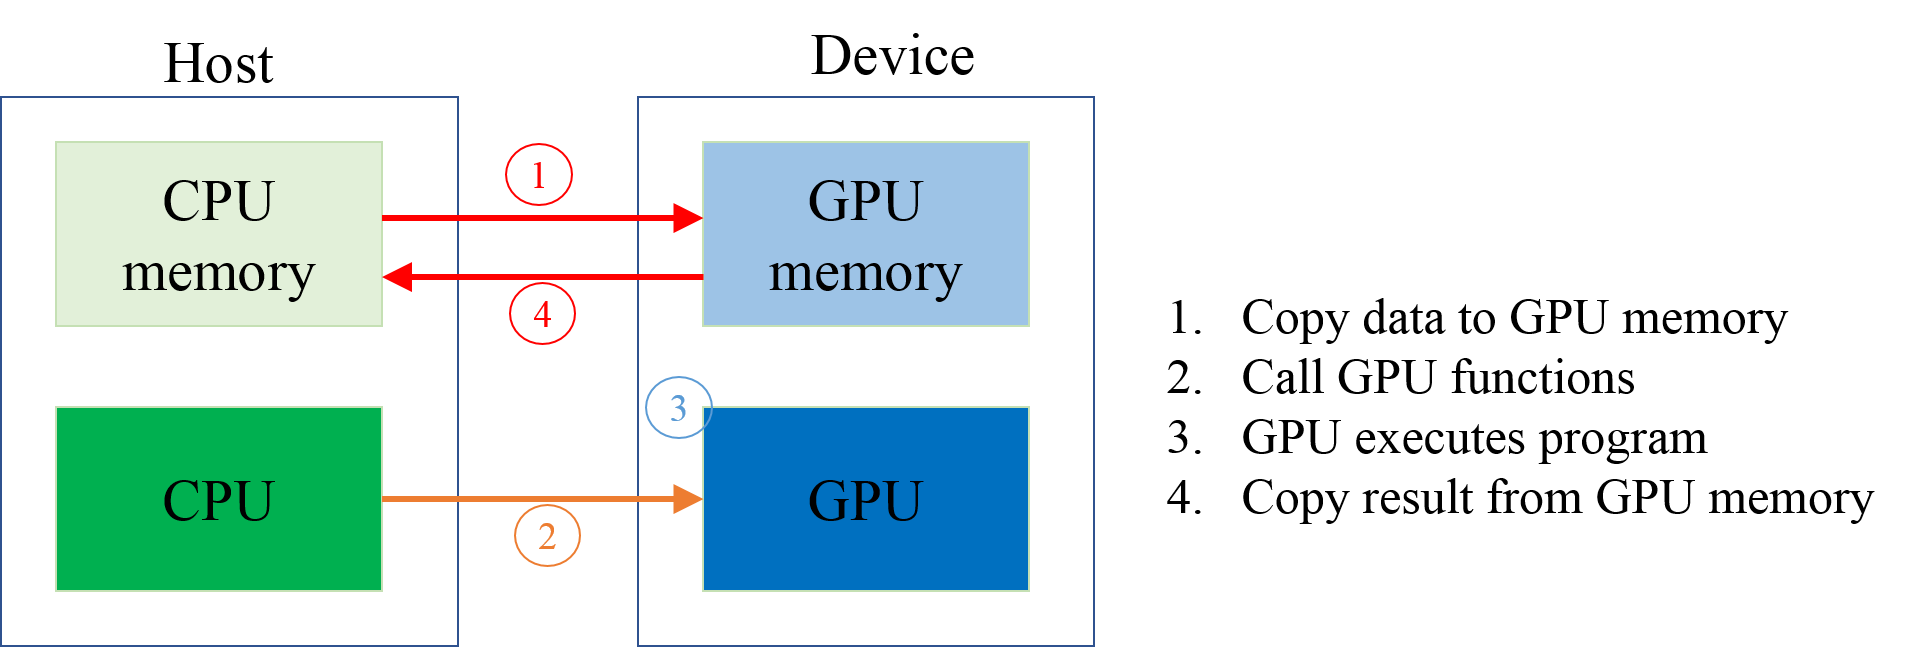
\includegraphics[scale=0.5]{image/fig_2_4}
    \caption{The simple flow chart of CUDA programming}
    \label{fig:fig_2_4}
\end{figure}

When the kernel is launched from the host, system creates many threads on GPU that executes simultaneously. The threads share the same program counter in the same warp. A warp consists 32 threads; warps are grouped into a block; blocks are grouped into a grid.

The \_\_shfl intrinsics permit exchanging of a variable between threads within a warp without use of shared memory. The exchange occurs simultaneously for all active threads within the warp (and named in mask), moving 4 or 8 bytes of data per thread depending on the type. Threads may only read data from another thread which is actively participating in the \_\_shfl command. If the target thread is inactive, the retrieved value is undefined.

Another keyword is atomic. An atomic function performs a read-modify-write atomic operation on one 32-bit or 64-bit word residing in global or shared memory. The operation is atomic in the sense that it is guaranteed to be performed without interference from other threads. In other words, no other thread can access this address until the operation is complete. Atomic functions do not act as memory fences and do not imply synchronization or ordering constraints for memory operations.

The more detail can be found on cuda programming guide \cite{cuda_programming_guide}.

\section{Related research}
Polygon operation is an important technique in Geographic Information Systems (GISs) and Very-Large-Scale-Integration (VLSI) design. In general polygon union, the common method is overlay polygons and calculate the generated polygons. Oosterom \cite{Peter:1994} presented a vector map-overlay algorithm used R-tree. Boost \cite{Simonson2009GeometryTL} \cite{Schling:2011:BCL:2049814} provides open source library to do the basic polygon operations. However, it is usually time consuming. Parallel algorithms used in VLSI design bring significant challenges for their efficient and effective implementation. Prasad et. al. \cite{Prasad:2015:GPR:2863697.2864578} presented a space-efficient data structure design and a non-trivial bottom-up construction algorithm for R-tree on GPUs. McKenney et. al. \cite{McKenney:2011:GOC:2093973.2094051} used a brute force approach to compute the line segment intersection. Wang et. al. presented a hybrid CPU-GPU approach which can be used to find the intersection and union of polygons represented in pixel format.

The plane sweep algorithm has also received many investigations since it forms the foundation of many common spatial operations, e.g. rectangle intersection in polygon operations and line segment intersection.
In 2009, McKenney et. al. \cite{McKenney2009APP} presented a parallel version of the plane sweep algorithm, which targeted towards the small number of processing cores available on commonly available multi-core systems. The overall design of their algorithm has three steps: (1) an initial scan equally slices the input data into p strips; (2) plane sweep algorithms run over each strip in parallel; (3) the result of the plane sweeps are merged into a result. Qiu et. al. \cite{Qiu2013APS} used Message-Passing-Interface (MPI) as the programming model, which is commonly used in the distributed memory architecture, to compute the line segments intersection by efficient and robust parallel plane sweep algorithm. Khlopotine et. al. \cite{Khlopotine2013AVO} presented a variant of a plane sweep algorithm to calculate the rectangle intersection and used OpenMP to enable parallel execution of the algorithm. Lo et. al. \cite{Lo2013OptimizingPB} provided a parallel algorithm to perform Pairwise Box Intersection checking on GPUs (PBIG). The PBIG algorithm consists of three phases: planning, mapping and checking. The planning phase partitions the space into small cells, the sizes of which are determined to optimize performance. The mapping phase maps the rectangles into the cells. The checking phase examines the rectangles intersections in the same cell. Several performance optimization techniques, including load-balancing, output data compression/encoding, and pipelined execution, are presented in the paper.
